\section{Entry and incumbent value: Whinston and Collins (1992)}\label{sec:09-wc}

The pricing regressions of \cref{sec:09-borenstein} infer market power from the cross-section of
fares. They need controls for demand and cost on every route, and they treat routes as unrelated
although each route is part of a network. \citet{WhinstonCollins1992} approach the same questions
from the stock market.\footnote{Page and footnote numbers in this section refer to the journal pages of
the article, and table numbers to its tables.} They ask how investors revalued incumbent airlines on the days People Express
announced entry into their markets. A fall in an incumbent's value reveals rents on the route before
entry, or sunk costs that keep the incumbent there after entry. Perfect contestability rules out both
(\cref{sec:09-contest}).

This section first develops the event-study method in general form (\cref{sec:09-wc-method}). It then
follows the paper in the order used for every case study in this book. We take up the question and its
logic, the setting and data, and the estimating equations. Then come the results on value, the price
and capacity responses to entry, and finally interpretation, limitations and contribution.

\subsection{Event-study methodology}\label{sec:09-wc-method}

An \emph{event study} measures the effect of a discrete piece of news on the market value of a firm.
The method goes back to \citet{FamaEtAl1969}, and \citet{BrownWarner1985} and \citet{MacKinlay1997} are
standard references. In industrial organization it was
used early to measure the effects of regulation \citep{Schwert1981,Rose1985}. We present the method
with general notation and then specialize it to the abnormal-dollar form that Whinston and Collins
use.

The premise is \emph{market efficiency}. The equity value of a firm equals the expected present value
of the cash flows to its shareholders, given all public information. News that changes expected
future profits therefore changes the share price as soon as it becomes public. The change in value in
a short window around the news, net of the return the stock would have earned anyway, measures the
change in expected discounted profits.

\casehead{Normal returns and the market model}
Index trading days by $\tau$ and firms by $f$. Let $R_{f\tau}$ be the return on firm $f$'s stock on
day $\tau$, including dividends. Let $R^0_\tau$ be the risk-free rate and $R^m_\tau$ the return on the
market portfolio. We work with \emph{excess returns} $r_{f\tau}\equiv R_{f\tau}-R^0_\tau$ and
$r^m_\tau\equiv R^m_\tau-R^0_\tau$. The \emph{normal return} is the return expected in the absence of
the event, and a model of it is the first ingredient of every event study.

\begin{assumption}[Market model]\label{ass:09-wc-mm}
For each firm $f$ and day $\tau$,
\begin{equation}\label{eq:09-wc-mm}
r_{f\tau} = a_f + b_f\, r^m_\tau + u_{f\tau},
\end{equation}
with $\E[u_{f\tau}\mid r^m]=0$, $\Var(u_{f\tau}\mid r^m)=\sigma_f^2$, and
$\Cov(u_{f\tau},u_{f\tau'}\mid r^m)=0$ for $\tau\neq\tau'$, where $r^m$ is the vector of market
excess returns on all days.
\end{assumption}

The coefficient $b_f$ is the firm's \emph{beta}, its exposure to market-wide news. The capital asset
pricing model (CAPM) implies $a_f=0$ and $b_f=\frac{\Cov(r_{f\tau},r^m_\tau)}{\Var(r^m_\tau)}$. The
market model leaves $a_f$ free, which guards against small errors in the pricing model. In this section
$a_f$ denotes this intercept. It does not denote the carrier effects of Borenstein's pricing equation. The errors may
be correlated across firms on the same day. This possibility matters when several firms are affected by
the same news, and we return to it below.

\casehead{Estimation and event windows}
An event $k$ affects firm $f$ and becomes public on trading day $\tau_k$, the \emph{announcement
day}. The \emph{event window} is a short set of days around $\tau_k$,
$\mathcal{W}_k=\{\tau_k-w^-,\dots,\tau_k+w^+\}$, with $w=w^-+w^++1$ days. Days before
$\tau_k$ allow for leakage of the news, and days after it allow for slow absorption. The
\emph{estimation window} $\mathcal{T}_0$ is a set of $L_0$ days that contains no event, usually a
long period before $\mathcal{W}_k$. On $\mathcal{T}_0$ we estimate \eqref{eq:09-wc-mm} by ordinary
least squares (OLS):
\begin{align*}
\hat b_f &= \frac{\sum_{\tau\in\mathcal{T}_0}(r^m_\tau-\bar r^m)(r_{f\tau}-\bar r_f)}
                 {\sum_{\tau\in\mathcal{T}_0}(r^m_\tau-\bar r^m)^2},\\
\hat a_f &= \bar r_f-\hat b_f\,\bar r^m,
\end{align*}
where $\bar r_f$ and $\bar r^m$ are means over $\mathcal{T}_0$. The residual variance estimate is
$\hat\sigma_f^2=\frac{1}{L_0-2}\sum_{\tau\in\mathcal{T}_0}(r_{f\tau}-\hat a_f-\hat b_f r^m_\tau)^2$.

\begin{definition}[Abnormal and cumulative abnormal returns]\label{def:09-wc-ar}
The \emph{abnormal return} of firm $f$ on a day $\tau\in\mathcal{W}_k$ is the prediction error
\begin{equation*}
\widehat{AR}_{f\tau} = r_{f\tau}-\hat a_f-\hat b_f\, r^m_\tau .
\end{equation*}
The \emph{cumulative abnormal return} over the window is
$\widehat{CAR}_{fk}=\sum_{\tau\in\mathcal{W}_k}\widehat{AR}_{f\tau}$.
\end{definition}

Under the null hypothesis that the event has no effect, \eqref{eq:09-wc-mm} also holds on the window
days. Substituting it into the definition gives the decomposition
\begin{equation*}
\widehat{AR}_{f\tau} = u_{f\tau}-(\hat a_f-a_f)-(\hat b_f-b_f)\,r^m_\tau .
\end{equation*}
The first term is the true error on day $\tau$. The other two terms are estimation error from
$\mathcal{T}_0$. We compute the variance conditional on market returns in four steps. First, write the
fitted normal return as $\hat a_f+\hat b_f r^m_\tau=\bar r_f+\hat b_f(r^m_\tau-\bar r^m)$. Second,
use the OLS results $\Var(\bar r_f)=\frac{\sigma_f^2}{L_0}$, $\Var(\hat b_f)=\frac{\sigma_f^2}{S_m}$
with $S_m=\sum_{s\in\mathcal{T}_0}(r^m_s-\bar r^m)^2$, and $\Cov(\bar r_f,\hat b_f)=0$. Third, note that
$u_{f\tau}$ for $\tau\in\mathcal{W}_k$ is uncorrelated with the estimation-window errors. Fourth, add
the pieces:
\begin{equation}\label{eq:09-wc-arvar}
\Var\big(\widehat{AR}_{f\tau}\mid r^m\big)
 = \sigma_f^2\left[1+\frac{1}{L_0}+\frac{(r^m_\tau-\bar r^m)^2}{S_m}\right].
\end{equation}
The bracket exceeds one only through estimation error, which vanishes as $L_0$ grows. For long
estimation windows we use $\Var(\widehat{AR}_{f\tau})\approx\sigma_f^2$ and
$\Var(\widehat{CAR}_{fk})\approx w\,\sigma_f^2$. The test statistic for one event is then
\begin{equation*}
z_{fk}=\frac{\widehat{CAR}_{fk}}{\hat\sigma_f\sqrt{w}},
\end{equation*}
which is approximately standard normal under the null when the daily errors are normal and $L_0$ is
large. With normal errors and a moderate $L_0$, it is approximately a $t$ variable with $L_0-2$ degrees of
freedom.

\casehead{Many events and clustered calendar dates}
With $K$ events the natural statistic is the average
$\overline{CAR}=\frac{1}{K}\sum_{k=1}^{K}\widehat{CAR}_k$. Its variance is
\begin{equation*}
\Var\big(\overline{CAR}\big)=\frac{1}{K^2}\left[\sum_{k}\Var\big(\widehat{CAR}_k\big)
 +\sum_{k\neq k'}\Cov\big(\widehat{CAR}_k,\widehat{CAR}_{k'}\big)\right].
\end{equation*}
Suppose the events fall on different calendar dates and the errors of different firms on different days
are uncorrelated. The covariances then vanish up to estimation-error terms of order
$\frac{\sigma_f^2}{L_0}$. The usual test then divides $\overline{CAR}$ by
$\frac{1}{K}\sqrt{\sum_{k}\Var\big(\widehat{CAR}_k\big)}$, which is the standard deviation of the average
when the covariances are zero.
When events cluster on the same dates, the covariances are not zero. Firms in one industry share
industry news that the market return does not absorb. Suppose $K$ firms are hit on the same days, each
with $\Var(\widehat{CAR}_k)=w\sigma^2$, and every pair of errors has correlation $\rho$. In this
paragraph only, $\rho$ denotes this correlation rather than a pass-through rate. Then
\begin{align*}
\Var\big(\overline{CAR}\big) &= \frac{1}{K^2}\big[K w\sigma^2+K(K-1)\rho\, w\sigma^2\big]\\
 &= \frac{w\sigma^2}{K}\big[1+(K-1)\rho\big].
\end{align*}
With $K=10$ and $\rho=0.3$ the variance is $3.7$ times the value that assumes independence. Ignoring
the correlation would overstate the precision of the estimate. Whinston and Collins face exactly this
problem, because each entry announcement hits several airlines on the same day.

\casehead{The dummy-variable form}
The two-step procedure has an equivalent one-step form. We estimate a single regression on
$\mathcal{T}_0\cup\mathcal{W}_k$ and add an indicator for each window day:
\begin{equation}\label{eq:09-wc-dummy}
r_{f\tau}=a_f+b_f\,r^m_\tau+\sum_{s\in\mathcal{W}_k}\gamma_{fs}\,\indic\{\tau=s\}+u_{f\tau}.
\end{equation}

\begin{proposition}[Equivalence of the two forms]\label{prop:09-wc-dummy}
OLS on \eqref{eq:09-wc-dummy} gives the estimation-window estimates $(\hat a_f,\hat b_f)$, and
$\hat\gamma_{fs}=\widehat{AR}_{fs}$ for every $s\in\mathcal{W}_k$. Under the null of no event effect,
the variance of $\hat\gamma_{fs}$ equals \eqref{eq:09-wc-arvar}.
\end{proposition}

\begin{proof}
The OLS objective splits into window days and estimation days:
\begin{equation*}
\sum_{s\in\mathcal{W}_k}\big(r_{fs}-a-b\,r^m_s-\gamma_{s}\big)^2
+\sum_{\tau\in\mathcal{T}_0}\big(r_{f\tau}-a-b\,r^m_\tau\big)^2 .
\end{equation*}
Each $\gamma_s$ appears in one squared term only. For any $(a,b)$, the choice
$\gamma_s=r_{fs}-a-b\,r^m_s$ sets that term to zero, which is its minimum. The remaining objective is
the sum over $\mathcal{T}_0$, which is minimized by the estimation-window OLS estimates. Hence
$\hat\gamma_{fs}=r_{fs}-\hat a_f-\hat b_f r^m_s=\widehat{AR}_{fs}$. Under the null, $\hat\gamma_{fs}$
equals the decomposition of $\widehat{AR}_{fs}$ given above, so its variance is
\eqref{eq:09-wc-arvar}.
\end{proof}

Summing the coefficients gives the cumulative abnormal return, $\sum_s\hat\gamma_{fs}=\widehat{CAR}_{fk}$,
and the regression delivers its standard error directly. A restricted version uses a single
indicator equal to one on all $w$ window days. Its coefficient is then close to the average daily
abnormal return, and $w$ times the coefficient estimates the cumulative effect. The match is not
exact, because the window days now also enter the estimate of $b_f$. The difference vanishes when
$L_0$ is large relative to $w$. The regression form has two further advantages. It allows the event
effect to depend on firm characteristics, and it allows many firms and events to be estimated jointly.
Whinston and Collins use both features.

\casehead{Systems of firms and seemingly unrelated regressions}
Stack the equations of $N_c$ firms for day $\tau$ as $y_\tau=X_\tau\theta+u_\tau$. Here $y_\tau$ is
the $N_c\times1$ vector of excess returns and $\theta$ stacks all parameters. The matrix $X_\tau$
collects each firm's regressors, with zeros in the positions of other firms' parameters. A system of
\emph{seemingly unrelated regressions} (SUR) assumes
\begin{equation*}
\E[u_\tau u_\tau^\top]=\Sigma,\qquad \E[u_\tau u_{\tau'}^\top]=0\quad\text{for }\tau\neq\tau',
\end{equation*}
so errors are correlated across firms on the same day but not across days \citep{Zellner1962}. The
generalized least squares (GLS) estimator and its variance are
\begin{align*}
\hat\theta_{GLS} &= \Big(\sum_\tau X_\tau^\top\Sigma^{-1}X_\tau\Big)^{-1}
                    \sum_\tau X_\tau^\top\Sigma^{-1}y_\tau,\\
\Var\big(\hat\theta_{GLS}\big) &= \Big(\sum_\tau X_\tau^\top\Sigma^{-1}X_\tau\Big)^{-1}.
\end{align*}
Feasible GLS replaces $\Sigma$ by $\hat\Sigma=\frac{1}{N_d}\sum_\tau\hat u_\tau\hat u_\tau^\top$,
built from equation-by-equation OLS residuals over the $N_d$ trading days. \Cref{sec:A-systems} reviews the
estimator.

\begin{remark}[When SUR matters]\label{rem:09-wc-sur}
If every equation has the same regressors and no parameter is shared across equations, GLS reduces to
OLS equation by equation \citep{Zellner1962}. Neither condition holds in the application below. The
regressors differ across firms, because they are scaled by each firm's own equity value and exposure.
The key parameters are common to all firms, which is a cross-equation restriction. SUR then gains
efficiency, it weights volatile stocks less, and its standard errors account for the correlation of
same-day errors across firms hit by the same event.
\end{remark}

\casehead{Choice of window}
A longer window captures more of the event's effect, including news that leaks before the
announcement. It also adds the noise of unrelated news on each extra day. With a window that ends on
the announcement day, $w^+=0$ and $\mathcal{W}_k=\{\tau_k-w+1,\dots,\tau_k\}$. Whinston and Collins
use one-, two- and three-day windows of this form (p.~450). In early work they also tried a
three-day window centered on the announcement day and found no information arriving after it
(n.~19). \Cref{fig:09-wc-timeline} shows the windows.

\begin{figure}[htbp]
\centering
\begin{tikzpicture}[x=1cm,y=1cm,
  win/.style={line width=3.2pt, blue!55!black, line cap=round},
  cwin/.style={line width=1.2pt, orange!80!black, dashed},
  lab/.style={font=\footnotesize, anchor=east},
  tick/.style={font=\scriptsize}]
\draw[-{Stealth[length=2.4mm]}, thick] (0,0) -- (14.6,0);
\node[font=\footnotesize, below] at (13.95,-0.14) {trading day $\tau$};
\fill[gray!25] (0.15,-0.12) rectangle (6.6,0.12);
\fill[gray!25] (13.35,-0.12) rectangle (13.95,0.12);
\draw[decorate, decoration={brace, mirror, amplitude=5pt}] (0.15,-0.25) -- (6.6,-0.25)
  node[midway, below=6pt, font=\footnotesize, align=center]
  {estimation period: trading days outside every window\\(the market model is fit here)};
\node at (7.05,0.32) {$\cdots$};
\node at (12.9,0.32) {$\cdots$};
\foreach \x/\tl in {8/{\tau_k-3}, 9/{\tau_k-2}, 10/{\tau_k-1}, 11/{\tau_k}, 12/{\tau_k+1}} {
  \draw (\x,0.1) -- (\x,-0.1);
  \node[tick, below] at (\x,-0.12) {$\tl$};
}
\draw[densely dotted, gray!60!black] (11,0.1) -- (11,2.25);
\node[font=\footnotesize, align=center] at (11,2.6) {announcement day $\tau_k$\\(earliest published report)};
\draw[win] (10.65,0.55) -- (11.35,0.55);
\node[lab] at (10.45,0.55) {one-day window};
\draw[win] (9.65,0.95) -- (11.35,0.95);
\node[lab] at (9.45,0.95) {two-day window};
\draw[win] (8.65,1.35) -- (11.35,1.35);
\node[lab] at (8.45,1.35) {three-day window};
\draw[cwin] (9.65,1.75) -- (12.35,1.75);
\node[lab] at (9.45,1.75) {centered window (check only)};
\end{tikzpicture}
\caption{Event windows for an announcement on trading day $\tau_k$. Solid bars are the one-, two- and
three-day windows that end on the announcement day. The dashed bar is the centered three-day window
used only to check for information arriving after the announcement. The market-model parameters are
estimated from the days outside all windows.}
\label{fig:09-wc-timeline}
\end{figure}

\casehead{Abnormal dollar values}
The standard event study measures the effect of an event as a return. Whinston and Collins argue that
the effect of their events is better measured in dollars (p.~449). The dollar loss from being an
incumbent in one entered market should depend on that market's profits, and not on the overall size
of the carrier. A loss of \$5 million is a return of $-2$ percent for a firm worth \$250 million and
$-0.2$ percent for a firm worth \$2.5 billion. A model with a common abnormal return would force the
larger carrier's dollar loss to be ten times larger. We now derive the return equation implied by a
dollar effect. \citet{WhinstonCollins1990} give a formal derivation from the CAPM, and we give the
simple version.

Let $V_{f\tau}$ be the market value of firm $f$'s equity at the end of day $\tau$ and $D_{f\tau}$ the
dividends it pays on day $\tau$. With a constant number of shares, the return is
\begin{equation*}
R_{f\tau}=\frac{V_{f\tau}+D_{f\tau}-V_{f,\tau-1}}{V_{f,\tau-1}},
\end{equation*}
so the dollar gain to shareholders on day $\tau$ is $G_{f\tau}\equiv V_{f\tau}+D_{f\tau}-V_{f,\tau-1}=
V_{f,\tau-1}R_{f\tau}$. We build $G_{f\tau}$ in three steps.

\emph{Step 1 (normal gain).} On a day without events, the CAPM gives
$R_{f\tau}=R^0_\tau+b_f(R^m_\tau-R^0_\tau)+u_{f\tau}$. Multiplying by $V_{f,\tau-1}$,
\begin{equation*}
G_{f\tau}=V_{f,\tau-1}\big[R^0_\tau+b_f(R^m_\tau-R^0_\tau)\big]+V_{f,\tau-1}u_{f\tau}.
\end{equation*}
The normal dollar gain and its noise both scale with the value of the firm.

\emph{Step 2 (event gain).} Let $\indic_\tau$ equal one if some event occurs on day $\tau$. Let
$\Delta_f(Z_\tau)$ be the expected dollar change in firm $f$'s value from the events of day $\tau$,
whose characteristics are collected in $Z_\tau$. Allow also a constant daily abnormal dollar gain
$a_f$, which absorbs small errors in the pricing model. Then
\begin{equation*}
G_{f\tau}=V_{f,\tau-1}\big[R^0_\tau+b_f(R^m_\tau-R^0_\tau)\big]+a_f+\indic_\tau\,\Delta_f(Z_\tau)
+V_{f,\tau-1}u_{f\tau}.
\end{equation*}
The event adds a fixed dollar amount that does not scale with $V_{f,\tau-1}$.

\emph{Step 3 (divide by value).} Dividing by $V_{f,\tau-1}$ and subtracting $R^0_\tau$ from both sides
gives
\begin{equation}\label{eq:09-wc-dollar}
R_{f\tau}-R^0_\tau=a_f\,\frac{1}{V_{f,\tau-1}}+b_f\big(R^m_\tau-R^0_\tau\big)
+\indic_\tau\,\frac{\Delta_f(Z_\tau)}{V_{f,\tau-1}}+u_{f\tau}.
\end{equation}
This is equation~(1) of \citet{WhinstonCollins1992}, where the error $u_{f\tau}$ is serially
uncorrelated. In return units the event effect is $\frac{\Delta_f(Z_\tau)}{V_{f,\tau-1}}$, so a fixed
dollar loss is a larger return for a smaller firm. The intercept also enters in dollars. As a check,
the authors re-estimated every specification with an added firm-specific constant in return units,
and the estimated value changes were nearly identical (n.~8). They also allowed the dollar
effect to differ across firms, and equality was not rejected (nn.~6 and~32). Both checks support
the dollar formulation.

\casehead{Identifying assumptions}
The event-study estimate measures the change in expected discounted profits only under the following
conditions.
\begin{enumerate}[label=(E\arabic*)]
\item \emph{Efficiency.} Prices incorporate public news within the window.
\item \emph{Correct dating and surprise.} The news first reaches the market inside the window, and it
was not anticipated before the window.
\item \emph{No confounding news.} No other news inside the window moves the same firms in a way
correlated with their exposure to the event.
\item \emph{Normal-return model.} Equation \eqref{eq:09-wc-mm} (or its dollar form) describes returns
outside the events, with stable $b_f$ and serially uncorrelated errors. Contemporaneous correlation
across firms is allowed.
\item \emph{Equity captures the change.} The change in firm value accrues to shareholders, rather than
being shared with debtholders or workers.
\end{enumerate}
Failures of (E2) and (E5) bias the estimates toward zero. \Cref{rem:09-anticipation} makes this
precise for anticipation. If investors had assigned probability $\varphi_0$ to entry before the
announcement, the measured change in value is only $(1-\varphi_0)L$, a fraction of the true loss $L$.
\Cref{sec:A-eventstudy} treats the general method and its pitfalls.

\subsection{Question, logic, and setting}\label{sec:09-wc-question}

Whinston and Collins pose two questions. The first is whether airline routes carry route-specific
profits or sunk costs, which is a test of the contestable-market model of
\citet{BaumolPanzarWillig1982}. The second is how localized airline competition is. Competition might
operate at the level of the airport pair, the city pair, or the whole network. Both questions matter
for the merger policy debates of 1986--1987 described in \cref{sec:09-hubs}.

Earlier evidence came from pricing studies \citep{GrahamKaplanSibley1983,CallKeeler1985,
BaileyGrahamKaplan1985,MorrisonWinston1987,Borenstein1989}. These studies regress route fares on
demand and cost proxies and on measures of market structure. Whinston and Collins name two weaknesses.
The studies treat routes as unrelated although each belongs to a network, and they need convincing
controls for demand and cost. Without good instruments, market structure is likely correlated with
unobserved demand and cost conditions (p.~446). Stock-market reactions to entry avoid both
problems, at the price of the assumptions (E1) to (E5).

\casehead{The logic}
The test rests on \cref{prop:09-valueloss}. An incumbent that loses value $L$ at an unanticipated entry
announcement must have had $V^0+K\ge L$. It earned positive economic profits on the route before entry,
or it had sunk costs that keep it there despite the loss, or both. A perfectly contestable market has $V^0=0$ and $K=0$, so it
implies $L\le0$. A significant value loss for incumbents therefore rejects contestability. In the
authors' words, the losses ``provide a lower bound on the level of profits or sunk costs existing in
these markets prior to entry'' (p.~447). The remarks that follow \cref{prop:09-valueloss} add three
refinements. The bound holds even though People Express had lower costs than the incumbents
(\cref{rem:09-lowcost}). Losses confined to incumbents of the entered route show that rents are tied to
that route (\cref{rem:09-localization}). Anticipation makes the measured loss a lower bound
(\cref{rem:09-anticipation}).

\casehead{Why People Express}
The authors chose entry by a single carrier for two reasons (pp.~446--447). First, industry observers saw
People Express as the embodiment of postderegulation innovations in product and cost (\cref{sec:09-hubs}).
If all events share this common driving force, they should have similar effects on airline values. Second,
the predictions are clear. By \cref{prop:09-entry-source}, entry triggered by an entrant's own innovation
lowers incumbents' values, while entry triggered by a common demand or cost shock can raise or lower them
(n.~4). An announcement driven by People Express's own innovation carries mostly bad news for incumbents,
which makes the sign of the effect interpretable.

\casehead{The setting}
People Express was a low-frill carrier based at Newark airport. Its 24 entry events of 1984 and 1985 all
involved airports without slot controls, and 22 of them involved Newark (\cref{sec:09-hubs}). Its stock
traded over the counter, so its own value can be tracked through the events (n.~15). The authors exclude airport pairs at the four slot-constrained airports listed in
\cref{sec:09-dominance-sources} and international routes, where regulation limits access (n.~9).

The choice of 1984 and 1985 has three advantages (p.~450). Six years had passed since the
Airline Deregulation Act of 1978. Nearly all flight restrictions imposed after the 1981 strike of air
traffic controllers (PATCO) had been lifted. Only Denver and Los Angeles were still constrained in
1984, and no event involves them while constrained (n.~10). Finally, the period precedes the
merger wave.

\subsection{Data}\label{sec:09-wc-data}

The study needs four kinds of information: the dates of the events, the incumbents in each entered
market, daily stock returns for a panel of airlines, and the airlines' operations.

\casehead{Events}
The authors searched \emph{Aviation Daily}, \emph{The Wall Street Journal} and \emph{The New York
Times} for every report of People Express entry. They read every 1984 and 1985 issue of
\emph{Aviation Daily}, which reached New York on the morning of its publication date (n.~11).
The event date is the publication date of the earliest report making clear that People Express would
enter the route. Usually this is the first report of People Express's own announcement. In three
cases it is an \emph{Aviation Daily} ``Intelligence Column'' report. \Cref{tab:09-wc-events} lists the
24 events. By our count they fall on 17 distinct dates, with up to three events on one date, so the
model must allow several events per day.

\begin{table}[htbp]
\centering
\caption{The 24 People Express entry events, 1984--1985}
\label{tab:09-wc-events}
\footnotesize
\begin{tabular}{@{}llll@{\hspace{1.4em}}lll@{}}
\toprule
Date & Airport pair & Source & & Date & Airport pair & Source\\
\midrule
1984-05-10 & EWR-Minneapolis    & AD           & & 1985-04-11 & EWR-Birmingham        & AD$^{b}$\\
1984-08-17 & EWR-Miami          & AD, NYT, WSJ & & 1985-04-17 & EWR-Raleigh/Durham    & AD$^{c}$\\
1984-08-17 & EWR-Detroit        & AD, NYT, WSJ & & 1985-04-17 & EWR-Charlotte         & AD$^{c}$\\
1984-09-10 & EWR-San Francisco  & WSJ$^{a}$    & & 1985-04-17 & EWR-Dayton            & AD$^{c}$\\
1984-09-10 & EWR-Denver         & WSJ$^{a}$    & & 1985-06-18 & EWR-Nashville         & AD, NYT\\
1984-10-03 & EWR-Cleveland      & AD, NYT, WSJ & & 1985-06-27 & EWR-Dallas/Ft.\ Worth & AD$^{b}$\\
1984-10-26 & EWR-Orlando        & AD$^{d}$     & & 1985-07-10 & EWR-Atlanta           & AD$^{b}$\\
1984-11-14 & Minneapolis-Tampa  & WSJ          & & 1985-07-17 & EWR-Albany            & AD, NYT\\
1984-11-28 & EWR-Greensboro     & AD, NYT, WSJ & & 1985-07-17 & EWR-Providence        & AD, NYT\\
1985-01-11 & EWR-Rochester      & AD           & & 1985-08-28 & Denver-San Diego      & AD, NYT, WSJ\\
1985-02-08 & EWR-Cincinnati     & AD           & & 1985-08-28 & EWR-New Orleans       & AD, NYT, WSJ\\
1985-04-10 & EWR-Ft.\ Lauderdale & AD          & & 1985-08-28 & EWR-St.\ Louis        & AD, NYT, WSJ\\
\bottomrule
\end{tabular}

\smallskip
\parbox{0.97\linewidth}{\footnotesize Notes: EWR is Newark. AD is \emph{Aviation Daily}, NYT
\emph{The New York Times}, WSJ \emph{The Wall Street Journal}. Dates are year-month-day.
(a) The report adds ``Probably also Cleveland and New Orleans.'' (b) \emph{Aviation Daily}
``Intelligence Column'' report that People Express would begin service. (c) Article saying People
Express was finalizing plans to serve these three markets. (d) ``Intelligence Column'' report that
People Express had secured a gate. Source: \citet{WhinstonCollins1992}, Appendix.}
\end{table}

\casehead{Market information}
For each event the authors read the \emph{Official Airline Guide} issue published just before the
event date. It lists every flight between two airports, by carrier and aircraft type. They recorded
each carrier's nonstop flights per week on the entered airport pair, and on all other airport pairs
in the same city pair. Only jet flights were counted. The only consequence is that Delta would have
been an incumbent in the Newark-Albany and Newark-Providence events had nonjet flights counted
(n.~13). Aircraft capacities convert flights into seats (n.~14). A \emph{seat-mile} is one
seat flown one mile, and a carrier's seat-miles on a route are its seats times the route distance.

\Cref{tab:09-wc-desc} collects the descriptive statistics that the paper reports. Five of the 24
events had no incumbent. The 19 events with incumbents averaged 1.68 incumbents, and the average over
all 24 events is $1.68\times\frac{19}{24}=1.33$, the figure the paper reports for the entered pair. The
average incumbent offered 7,100 seats per week on a route of average length 892 miles.

\begin{table}[htbp]
\centering
\caption{Descriptive statistics for the People Express events}
\label{tab:09-wc-desc}
\small
\begin{tabular}{@{}lrl@{}}
\toprule
Statistic & Value & Location\\
\midrule
Entry events (involving Newark) & 24 (22) & p.~450\\
Events with no incumbent on the entered pair & 5 & p.~451\\
Incumbents per event, events with incumbents (s.d.) & 1.68 (0.78) & p.~451\\
Seats per week, average incumbent (s.d.) & 7,100 (3,283) & p.~451\\
Distance of entered routes, miles (s.d.) & 892 (549) & p.~451\\
\addlinespace
Seat-miles per week, entered airport pair & 8,718,000 & p.~455\\
Seat-miles per week, other airports in the city pair & 21,860,000 & p.~455\\
Incumbents per event, entered pair & 1.33 & p.~455\\
Incumbents per event, other airports & 2.71 & p.~455\\
$\Pr(\mathit{OSM}>0\mid \mathit{SM}>0)$, all events & 0.719 & p.~455\\
$\Pr(\mathit{OSM}>0\mid \mathit{SM}>0)$, New York-area events & 0.793 & p.~455\\
\addlinespace
Share of departures at newly entered airport, carriers with $\mathit{SM}>0$ & 44.3\% & p.~456\\
Same, carriers with $\mathit{SM}>0$ or $\mathit{OSM}>0$ & 59.1\% & p.~456\\
Annual departures at newly entered airport, average carrier & 3,444 & fn.~26\\
Annual departures at newly entered airport, entered-pair incumbent & 29,616 & fn.~26\\
\addlinespace
Annual revenue per seat-mile, incumbents (weighted, \$) & 0.081 & p.~452\\
Firms in the stock panel, all exchanges & 20 & p.~451\\
\quad of which traded on NYSE or AMEX every day & 16 & p.~451\\
\quad of which traded over the counter & 4 & p.~451\\
\bottomrule
\end{tabular}

\smallskip
\parbox{0.97\linewidth}{\footnotesize Notes: $\mathit{SM}$ and $\mathit{OSM}$ are a carrier's seat-miles
on the entered airport pair and on other airport pairs of the same city pair. The departure shares
exclude the Minneapolis-Tampa event and condition on events with some incumbent. Revenue per seat-mile
weights each airline by its share of the seat-miles People Express entered against. Locations are
journal pages. Source: \citet{WhinstonCollins1992}.}
\end{table}

\casehead{Stock data}
Daily returns come from the CRSP tape for all airline stocks on the New York and American Stock
Exchanges. Sixteen carriers traded every day of the sample. The authors added four carriers traded
over the counter (OTC). The NYSE firms are American, Alaska Air, Delta, Eastern, Northwest Orient,
Pacific Southwest, Pan Am, Piedmont, Republic, Trans World, United, USAir and Western. The AMEX firms
are Continental, Ozark and Texas Air. The OTC firms are Air California, America West, Midway and
People Express (n.~15). Texas Air held the stock of Continental and New York Air. Its event variables are
combinations of those two airlines' variables, weighted by its ownership shares. Nearly all of each
firm's operations were in air transport. The exception is United, whose airline operations still
accounted for over five-eighths of its assets (n.~16).

\casehead{Unit of observation}
An observation is a firm on a trading day of 1984--1985. The dependent variable is the excess return
$R_{f\tau}-R^0_\tau$. There are $N_c=19$ carriers besides People Express, plus People Express itself.

\subsection{Estimating equations and specifications}\label{sec:09-wc-spec}

Each event $k$ has a set of measurable characteristics $Z^k_f$ for each carrier $f$, such as the
carrier's seats on the entered route. The dollar change in carrier $f$'s value from event $k$ is
modeled as a known function $g(Z^k_f;\Lambda)$ of these characteristics and a parameter vector
$\Lambda$. Whinston and Collins write this function as $f(Z^k_i,\Lambda)$, and we use $g$ because $f$
indexes firms. Let $E_\tau$ be the set of events whose window contains day $\tau$. The total dollar
change on day $\tau$ is
\begin{equation}\label{eq:09-wc-delta}
\Delta_f(Z_\tau)=\sum_{k\in E_\tau}g(Z^k_f;\Lambda).
\end{equation}
Substituting \eqref{eq:09-wc-delta} into \eqref{eq:09-wc-dollar}, and using $\indic_\tau=1$ exactly
when $E_\tau$ is nonempty, gives the basic estimating equation for carrier $f$:
\begin{equation}\label{eq:09-wc-main}
R_{f\tau}-R^0_\tau=a_f\,\frac{1}{V_{f,\tau-1}}+b_f\big(R^m_\tau-R^0_\tau\big)
+\sum_{k\in E_\tau}\frac{g(Z^k_f;\Lambda)}{V_{f,\tau-1}}+u_{f\tau}.
\end{equation}
The empty sum is zero on days without events, so the indicator is no longer needed. People Express
has its own equation, in which $g$ is replaced by a function $h(X^k;\lambda_{PE})$ of event
characteristics $X^k$. In every specification below, $h=\lambda_{PE}$, a constant dollar change per
event. The $N_c=19$ carrier equations and the People Express equation form a system with
contemporaneously correlated errors, estimated jointly as in \cref{rem:09-wc-sur}.

With a $w$-day window, event $k$ belongs to $E_\tau$ on each of the days $\tau_k-w+1,\dots,\tau_k$.
The coefficients then measure the average daily dollar change, and the paper reports $w$ times this
average as the total value change over the window (p.~452). All estimates below are totals in
this sense.

\casehead{Specification 1: incumbency on the entered pair}
The simplest specification makes each carrier's loss proportional to its seat-miles on the entered
route:
\begin{equation}\label{eq:09-wc-sm}
g(Z^k_f;\Lambda)=\lambda_{SM}\,\mathit{SM}^k_f .
\end{equation}
Here $\mathit{SM}^k_f$ is carrier $f$'s annualized seat-miles on the airport pair entered in event
$k$, equal to its weekly seat-miles just before the announcement times 52. The parameter
$\lambda_{SM}$ is the dollar change in value per annualized seat-mile. The paper calls it $\gamma$.

Two considerations motivate seat-miles (pp.~451--452). Within an event, it is natural that
each incumbent's loss is proportional to its share of the seats on the route. Across events, the total
loss of incumbents should grow with market size, measured by seats. Customer values and costs both
rise with distance, so a seat on a 2,000-mile route should carry a larger dollar effect than a seat on
a 200-mile route. Seat-miles combine the two. This choice matches industry practice of reporting
operating profit per available seat-mile (n.~17). The data allow no seasonal adjustment
(n.~18).

The authors note reasons why other forms might fit better. Longer routes may face more competition from
connecting service, so losses could fall with distance. If People Express entered at a scale
independent of market size, the total loss would not depend on seats. Effects could also be firm
specific. Footnote~32, reported with the results below, tests these alternatives.

\casehead{Specification 2: general effects}
An announcement could lower the values of carriers that are not incumbents on the entered route
(p.~454). Three channels are possible. Entry could set off competitive adjustments throughout
the network, including in regulated segments where rents are likely, such as slot-constrained airports
and international routes. Carriers own aircraft, and entry announcements may coincide with changes in
aircraft values. The announcement may also reveal information about the likely scale of People
Express's future expansion. To absorb such effects the authors add a firm fixed effect per event:
\begin{equation}\label{eq:09-wc-fe}
g(Z^k_f;\Lambda)=\lambda_f+\lambda_{SM}\,\mathit{SM}^k_f .
\end{equation}
The paper writes the fixed effect as $\alpha_i$, the same symbol as the intercept in
\eqref{eq:09-wc-dollar}. We write $\lambda_f$ to keep the two apart. If the general effect works
through slot values, $\lambda_f$ is related to the number of slots carrier $f$ holds. If it works
through information about future expansion, $\lambda_f$ is related to the probability that carrier $f$
is an incumbent in a later People Express event.

\casehead{Specification 3: other airports in the city pair}
Twenty-two events involve Newark, which competes to some extent with La Guardia and Kennedy for New
York traffic. Both of these airports are slot constrained, so carriers there may hold regulatory rents
that entry at Newark could erode. If Newark incumbents also tend to serve the same city from La Guardia
or Kennedy, the seat-mile variable could pick up losses that belong to those airports. The authors add
$\mathit{OSM}^k_f$, carrier $f$'s annualized seat-miles between the two cities of event $k$ at airport
combinations other than the entered pair:
\begin{equation}\label{eq:09-wc-osm}
g(Z^k_f;\Lambda)=\lambda_f+\lambda_{SM}\,\mathit{SM}^k_f+\lambda_{OSM}\,\mathit{OSM}^k_f .
\end{equation}
In all but 2 of the 24 events, the other seat-miles are slot-constrained departures from La Guardia or
Kennedy to the airport that People Express entered from Newark (p.~455). The paper's symbol
for $\lambda_{OSM}$ is $\phi$.

The other airports offered about two and a half times as many seat-miles as the entered pair
(\cref{tab:09-wc-desc}), mostly because they had more incumbents. Carriers often served both: the
probability that $\mathit{OSM}^k_f>0$ given $\mathit{SM}^k_f>0$ is 0.719 overall and 0.793 for New
York-area events. The contrast between $\lambda_{SM}$ and $\lambda_{OSM}$ is therefore identified
mainly by comparing carriers that serve both the entered pair and other airports with carriers that
serve only other airports. Without demand or cost differences between airports in the same city, the
two effects per seat-mile should be similar. Their difference measures differentiation between
airports.

\casehead{Specification 4: separate New York fixed effects}
Suppose slots at a constrained airport could be shifted freely across the markets served from it.
Then entry would lower the profit of every departure at that airport equally. Each carrier would bear
the same loss per slot, regardless of which city it serves, and $\mathit{OSM}$ would pick up little
of it (p.~455). The firm effects already absorb most of such a loss, since 22 events involve
Newark. To be safe, the authors allow separate firm effects for the two non-New York events:
\begin{equation}\label{eq:09-wc-nny}
g(Z^k_f;\Lambda)=\lambda_f+\lambda^{NNY}_f I^{NNY}_k+\lambda_{SM}\,\mathit{SM}^k_f
+\lambda_{OSM}\,\mathit{OSM}^k_f ,
\end{equation}
where $I^{NNY}_k=1$ if event $k$ is not in the New York area. The general effect is $\lambda_f$ in New
York events and $\lambda_f+\lambda^{NNY}_f$ elsewhere. Separate effects also absorb informational
losses that depend on whether People Express was expected to keep expanding from Newark.

\casehead{Specification 5: the newly entered airport}
In every event except Minneapolis-Tampa, People Express entered an airport for the first time. It
thereby also entered connecting city pairs between the new city and the rest of its network. Carriers
on those connecting routes could lose value too. Entered-pair incumbents held large shares at the newly
entered airport: 44.3 percent of its departures on average, and 59.1 percent including carriers with
$\mathit{OSM}>0$ (\cref{tab:09-wc-desc}). To separate route incumbency from airport presence, the
authors add $\mathit{EPORT}^k_f$, carrier $f$'s departures at the airport entered in event $k$, in the
year of the event. It is zero for all carriers in the Minneapolis-Tampa event (n.~27). The most
elaborate specification is
\begin{equation}\label{eq:09-wc-full}
g(Z^k_f;\Lambda)=\lambda_f+\lambda^{NNY}_f I^{NNY}_k+\lambda_{SM}\,\mathit{SM}^k_f
+\lambda_{OSM}\,\mathit{OSM}^k_f+\lambda_{EP}\,\mathit{EPORT}^k_f .
\end{equation}
The paper's symbol for $\lambda_{EP}$ is $\eta$.

\casehead{The estimating equation in full}
Substituting \eqref{eq:09-wc-full} into \eqref{eq:09-wc-main} shows that every specification is
linear in its parameters. Let $n_{\tau}=|E_\tau|$ be the number of events whose window contains day
$\tau$, and $n^{NNY}_{\tau}$ the number of those outside New York. Then
\begin{multline*}
R_{f\tau}-R^0_\tau=a_f\,\frac{1}{V_{f,\tau-1}}+b_f\big(R^m_\tau-R^0_\tau\big)
+\lambda_f\,\frac{n_\tau}{V_{f,\tau-1}}+\lambda^{NNY}_f\,\frac{n^{NNY}_\tau}{V_{f,\tau-1}}\\
+\lambda_{SM}\,\frac{\sum_{k\in E_\tau}\mathit{SM}^k_f}{V_{f,\tau-1}}
+\lambda_{OSM}\,\frac{\sum_{k\in E_\tau}\mathit{OSM}^k_f}{V_{f,\tau-1}}
+\lambda_{EP}\,\frac{\sum_{k\in E_\tau}\mathit{EPORT}^k_f}{V_{f,\tau-1}}+u_{f\tau}.
\end{multline*}
Each regressor is a predetermined exposure divided by the previous day's equity value. Linear SUR
applies directly.

\casehead{Identification}
The parameters are identified from two sources of variation. Event timing separates event days from
ordinary days, and the market model absorbs market-wide news on all days. Within event days, carriers
differ in their exposure to each event. A carrier that is not an incumbent anywhere in an event
reveals the general effect $\lambda_f$ through its returns on event days. Comparing incumbents with
non-incumbents on the same days, relative to each carrier's own general effect, identifies
$\lambda_{SM}$. The $\mathit{OSM}$ and $\mathit{EPORT}$ effects are identified because these exposures
are imperfectly correlated with $\mathit{SM}$. The price of this flexibility is precision. Each
$\lambda_f$ is estimated from about 17 event dates, and each $\lambda^{NNY}_f$ from two events.

\subsection{Results on value}\label{sec:09-wc-value}

\casehead{The simplest specification}
\Cref{tab:09-wc-t1} reproduces Table~1 of the paper, specification \eqref{eq:09-wc-sm} for the three
windows. Incumbents on the entered route lost between \$0.0109 and \$0.0191 of value per annualized
seat-mile. The effect is precise in every window. Dividing the rounded estimates by their standard
errors gives $t$ statistics of $-3.11$, $-3.00$ and $-3.13$. The paper reports a range of $-2.98$ to
$-3.15$, computed from unrounded estimates (p.~452).

\begin{table}[htbp]
\centering
\caption{Total value response to People Express entry, simplest specification}
\label{tab:09-wc-t1}
\small
\begin{tabular}{@{}lccc@{}}
\toprule
 & \multicolumn{3}{c}{Event window}\\
\cmidrule(l){2-4}
Variable & One-day & Two-day & Three-day\\
\midrule
Incumbent effect per annualized seat-mile, $\lambda_{SM}$ (\$) & $-0.0109$ & $-0.0147$ & $-0.0191$\\
 & (0.0035) & (0.0049) & (0.0061)\\
People Express effect, $\lambda_{PE}$ (\$1,000s) & $-354$ & $440$ & $-1{,}293$\\
 & (1,103) & (1,548) & (1,914)\\
\midrule
$t$ statistic for $\lambda_{SM}$ (computed from rounded entries) & $-3.11$ & $-3.00$ & $-3.13$\\
\bottomrule
\end{tabular}

\smallskip
\parbox{0.97\linewidth}{\footnotesize Notes: Specification \eqref{eq:09-wc-sm}, estimated by SUR on
the daily returns of 19 carriers and People Express, 1984--1985. Windows end on the announcement day.
Entries are total value changes over the window. Standard errors in parentheses. The last row is
computed by us. Source: \citet{WhinstonCollins1992}, Table~1.}
\end{table}

\casehead{Magnitudes}
The estimates translate into dollars as follows. The paper reports a loss per incumbent of \$3.7
million to \$6.5 million (p.~452). Dividing by the coefficients recovers the annualized
seat-miles of the average incumbent:
\begin{equation*}
\frac{\$3.7\text{ million}}{0.0109}\approx 339\text{ million},\qquad
\frac{\$6.5\text{ million}}{0.0191}\approx 340\text{ million seat-miles per year}.
\end{equation*}
The product of the mean seats and the mean distance gives a slightly smaller figure,
$7{,}100\times892\times52\approx329$ million, because the paper averages the product of seats and
distance over incumbents. Events with incumbents had 1.68 incumbents on average, so the loss per event
for all incumbents combined is
\begin{equation*}
1.68\times\$3.7\text{ million}\approx\$6.2\text{ million}\quad\text{to}\quad
1.68\times\$6.5\text{ million}\approx\$10.9\text{ million}.
\end{equation*}
These are after-tax losses to shareholders. At the 46 percent corporate tax rate of the period, the
pretax loss per incumbent is
\begin{equation*}
\frac{\$3.7\text{ million}}{1-0.46}\approx\$6.8\text{ million}\quad\text{to}\quad
\frac{\$6.5\text{ million}}{1-0.46}\approx\$12.0\text{ million}.
\end{equation*}

A second comparison scales the loss by revenue. The incumbents' weighted average annual revenue per
seat-mile was \$0.081 (n.~20). The pretax loss per seat-mile as a fraction of a year's revenue is
\begin{equation*}
\frac{0.0109}{0.54\times0.081}=\frac{0.0109}{0.0437}\approx0.25\quad\text{to}\quad
\frac{0.0191}{0.54\times0.081}=\frac{0.0191}{0.0437}\approx0.44 .
\end{equation*}
Here $0.54=1-0.46$ converts the after-tax loss per seat-mile into a pretax loss.
The paper reports 25 to 43 percent. An incumbent that flew its planes on the entered route completely
empty would lose its revenue while bearing the same costs. A loss of 0.25 to 0.44 years of revenue is
therefore comparable to flying the route empty for $0.25\times12=3$ to $0.44\times12\approx5$ months.
The authors conclude that route profits or sunk costs before entry were substantial.\footnote{The
paper's introduction rounds these figures to a loss of ``\$3 million to \$6 million'' per incumbent and
a pretax loss of ``\$6 million and \$12 million'' (p.~447). We use the figures of Section~4 of
the paper.}

\casehead{Biases}
The estimates could understate the true loss for three reasons (p.~453). Events may be
misdated, the market may have anticipated part of the news, and some of the loss may fall on
debtholders or on workers who share rents. A fourth reason concerns connecting traffic. A seat on the
entered route also serves connecting passengers, so the loss per seat averages the losses on the two
kinds of traffic. People Express entered mainly the city-pair market. To the extent that entry hurt
city-pair traffic more than connecting traffic, the loss per seat understates the loss in the
city-pair market. Entry can still hurt connecting traffic, through lost economies of density, reduced frequency,
or arbitrage between fares (n.~21). Reasons the estimates might overstate the loss motivate the
richer specifications below.

\casehead{People Express's own value}
The estimated changes in People Express's value are small, at most \$1.3 million in absolute value.
They are also imprecise, each within one standard error of zero, and of inconsistent
sign.\footnote{The paper describes them as below \$1 million in absolute value (p.~453). This holds for
the one- and two-day windows. The three-day estimate in its Table~1 is $-\$1.293$ million.} The authors
offer two readings (pp.~453--454). The scale of
expansion may have been fully anticipated, with only its location unknown. Then People Express's value
would not move while its targets lost value. This reading predicts zero expected loss for the set of
all possible incumbents, which the general effects below contradict. The panel lacks only one notable
possible incumbent, Frontier Airlines, so it comes close to that set (n.~22). Alternatively, the scale was
unanticipated, and each extra entry yielded People Express little return while lowering incumbents'
profits. Some observers thought that the move into major markets was a mistake. The test does not
require optimal entry choices. A low-price entrant reveals incumbents' sunk costs whether or not its
prices cover its own costs (n.~23).

\casehead{The richer specifications}
\Cref{tab:09-wc-t2} reproduces Table~2 of the paper, which adds the controls of specifications
\eqref{eq:09-wc-fe} to \eqref{eq:09-wc-full} for the one-day window. The results for two- and
three-day windows are similar and appear in \citet{WhinstonCollins1990}.

\begin{table}[htbp]
\centering
\caption{Total value response to entry, one-day window, five specifications}
\label{tab:09-wc-t2}
\small
\begin{tabular}{@{}lccccc@{}}
\toprule
Variable & (1) & (2) & (3) & (4) & (5)\\
\midrule
Airport-pair incumbent effect, $\lambda_{SM}$ & $-0.0109$ & $-0.0127$ & $-0.0158$ & $-0.0144$ & $-0.0126$\\
 & (0.0035) & (0.0040) & (0.0053) & (0.0054) & (0.0058)\\
Other airports incumbent effect, $\lambda_{OSM}$ & & & $0.0025$ & $0.0020$ & $0.0026$\\
 & & & (0.0028) & (0.0028) & (0.0029)\\
Entered airport effect, $\lambda_{EP}$ & & & & & $-33.8$\\
 & & & & & (38.2)\\
People Express effect, $\lambda_{PE}$ (\$1,000s) & $-354$ & $-256$ & $-262$ & $-268$ & $-262$\\
 & (1,103) & (1,144) & (1,144) & (1,144) & (1,144)\\
\addlinespace
Firm fixed effects $\lambda_f$ & No & Yes & Yes & Yes & Yes\\
Separate New York fixed effects $\lambda^{NNY}_f$ & No & No & No & Yes & Yes\\
\addlinespace
Sum of estimated fixed effects (\$1,000s) & & $-30{,}841$ & & & $-36{,}238$\\
 & & (17,621) & & & (19,136)\\
\bottomrule
\end{tabular}

\smallskip
\parbox{0.97\linewidth}{\footnotesize Notes: Column (1) is specification \eqref{eq:09-wc-sm} and
repeats the one-day column of \cref{tab:09-wc-t1}. Columns (2) to (5) are specifications
\eqref{eq:09-wc-fe}, \eqref{eq:09-wc-osm}, \eqref{eq:09-wc-nny} and \eqref{eq:09-wc-full}.
$\lambda_{SM}$ and $\lambda_{OSM}$ are dollars per annualized seat-mile. $\lambda_{EP}$ is dollars per
annual departure at the newly entered airport. Standard errors in parentheses. The fixed-effect sums
are reported only for columns (2) and (5). Source: \citet{WhinstonCollins1992}, Table~2.}
\end{table}

The incumbency effect survives every control. Its estimate rises slightly in absolute value, from
$-0.0109$ in column~(1) to $-0.0126$ in column~(5). Its precision falls, and the column~(5) $t$
statistic is $-2.18$ (our ratio of the rounded entries gives $-2.17$). The two- and three-day estimates
of specification \eqref{eq:09-wc-full} are $-0.0154$ (0.0082) and $-0.0142$ (0.0101). Their average
across the three windows,
\begin{equation*}
\frac{-0.0126-0.0154-0.0142}{3}=-0.0141,
\end{equation*}
is close to the average of the three columns of \cref{tab:09-wc-t1} (n.~28),
\begin{equation*}
\frac{-0.0109-0.0147-0.0191}{3}=-0.0149 .
\end{equation*}
The losses are tied to incumbency on the entered route.

\casehead{General effects}
The sum of the 19 estimated fixed effects in column~(5) is $-\$36.2$ million per event. Divided equally
among the 19 carriers, it is a general loss of $\frac{36{,}238}{19}\approx\$1.9$ million per carrier
and event. The column~(5) incumbency effect for the average incumbent is
$0.0126\times339\text{ million}\approx\$4.3$ million. An incumbent therefore loses about
$4.3+1.9=\$6.2$ million, more than three times the \$1.9 million loss of a non-incumbent (journal
p.~456). The general part is $\frac{1.9}{6.2}\approx30$ percent of an incumbent's loss.

The picture reverses for the industry. Per event, the incumbency loss of all incumbents together is
about $0.0126\times52\times8{,}718{,}000\approx\$5.7$ million. The general losses total
\$36.2 million. General effects are therefore $\frac{36.2}{36.2+5.7}\approx86$ percent of the industry
loss, ``over 80\%'' in the paper's words. Weighting the fixed effects by each carrier's extent of
incumbency gives a general loss of \$3.75 million for the average incumbent. On that basis an
incumbent loses $\frac{4.3+3.75}{3.75}\approx2.1$ times as much as a non-incumbent (n.~29). The
general effects fall more heavily on carriers that were more likely to be incumbents. Their source
remains unclear. Competitive spillovers through the network, aircraft values and information about
People Express's future scale are all consistent with them.

The non-New York fixed effects are not reported. They rest on two events only and are noisy. A
\emph{quasi-likelihood ratio test}, a likelihood-ratio-type test computed from the SUR objective, does not
reject equality of the New York and non-New York fixed effects at conventional levels (p.~457).

\casehead{Other airports in the city}
The $\mathit{OSM}$ effect is small, positive and insignificant in all three columns. It is an order of
magnitude smaller than the $\mathit{SM}$ effect.\footnote{The paper's text reads ``an order of
magnitude smaller than the OSM effect'' (p.~457). The intended comparison is with the SM
effect.} The two- and three-day estimates are $0.0028$ (0.0039) and $-0.0017$ (0.0048), so even the
sign is unstable (n.~30). The authors reject equality of the $\mathit{SM}$ and $\mathit{OSM}$
effects at the 2.5 percent level. For intuition, if the two column~(5) estimates were uncorrelated,
the difference $-0.0152$ would have standard error $\sqrt{0.0058^2+0.0029^2}\approx0.0065$ and a
$z$ statistic of $-2.34$. Airports in the same city are differentiated, on the demand side, the cost
side, or both. This finding agrees with the high value carriers placed on La Guardia and Kennedy
slots despite the existence of Newark.

The authors warn against reading the result as the absence of substitution between airports
(p.~457). Entry need not harm sellers of substitutes. People Express served mainly travelers
with a low willingness to pay. Its entry might lead the Newark incumbent to cut frequency or crowd its
coach cabin, or might make Newark less attractive in general. La Guardia carriers would then gain
business travelers, and the gain could exceed their loss of discount passengers (n.~31).

\casehead{The newly entered airport}
The $\mathit{EPORT}$ coefficient is negative, small and insignificant, $-33.8$ (38.2) dollars per annual
departure. For the average carrier, with 3,444 annual departures at the newly entered airport, it
implies a loss of $33.8\times3{,}444\approx\$0.12$ million. For entered-pair incumbents, with 29,616
departures, it implies $33.8\times29{,}616\approx\$1.0$ million. This is small next to their \$4.3
million loss from incumbency on the entered pair (p.~458).

\casehead{Robustness}
Footnote~32 reports two further checks for the one-day window. The first replaces $\mathit{SM}^k_f$ by
\begin{equation*}
\big[\lambda_0+\lambda_1\mathit{SEATS}_k+\lambda_2\mathit{DIST}_k+\lambda_{SM}\,\mathit{DIST}_k\,
\mathit{SEATS}_k\big]\,\mathit{SH}^k_f ,
\end{equation*}
where $\mathit{SEATS}_k$ and $\mathit{DIST}_k$ are the route's total seats and distance and
$\mathit{SH}^k_f$ is carrier $f$'s seat share on the entered pair. The same construction replaces
$\mathit{OSM}^k_f$. Specification \eqref{eq:09-wc-full} is the case $\lambda_0=\lambda_1=\lambda_2=0$. A test of
the six added parameters comes nowhere close to rejecting it. The most important added term is
distance. With it alone, the losses per seat-mile at the sample means are $-0.0118$ (0.0059) on the
entered pair and $-0.0009$ (0.0047) at other airports. The second check gives each firm its own
seat-mile coefficient in specification \eqref{eq:09-wc-sm}. Equality is not rejected, and the average
coefficient is $-0.0105$. A firm-specific constant in return units also leaves the estimates nearly
unchanged (n.~8).

\subsection{Price, quantity, and capacity responses}\label{sec:09-wc-did}

The stock market reveals expected losses. Section~5 of the paper asks what incumbents did after entry,
using prices, ticket sales and schedules. The evidence corroborates the value results and adds a
surprise about quantities.

\casehead{Data}
Prices and quantities come from the Department of Transportation's Origin and Destination Survey, a 10
percent sample of tickets, for the first quarters of 1984, 1985 and 1986 (n.~33). The outcomes are
year-to-year percentage changes in the mean coach price, in the standard deviation of coach prices,
and in coach tickets sold. Only New York-area events are used. Two events of the first quarter of 1985
are dropped, since their year of entry is ambiguous. By the dates in \cref{tab:09-wc-events}, these
are Rochester and Cincinnati. Nashville is dropped because it had no Newark incumbent in the first
quarter of 1984. San Francisco is dropped because People Express switched to another airport pair in
that city pair within a year. The data cover all direct flights between Newark and the new city,
including multistop flights without a change of plane. The final samples have 7 markets entered in
1984 and 8 entered in 1985.

\casehead{Design}
The design is a \emph{difference in differences} (\cref{sec:A-did}). Each cohort serves as the control for the other in
one period. Let $\ln P_{ty}$ be the log mean incumbent price in market $t$ in the first quarter of
year $y$. Let $D_{ty}=1$ if People Express announced entry into $t$ before that quarter. Consider the
model
\begin{equation}\label{eq:09-wc-did-model}
\ln P_{ty}=\mu_t+\nu_y+\varphi_E\,D_{ty}+e_{ty},
\end{equation}
with market effects $\mu_t$, year effects $\nu_y$ and a constant entry effect $\varphi_E$. For the 1984
cohort, $D$ is $(0,1,1)$ in 1984, 1985 and 1986. For the 1985 cohort it is $(0,0,1)$. First
differences remove the market effects:
\begin{equation*}
\ln P_{t,y+1}-\ln P_{ty}=(\nu_{y+1}-\nu_y)+\varphi_E\,(D_{t,y+1}-D_{ty})+(e_{t,y+1}-e_{ty}).
\end{equation*}
Comparing cohorts within a period removes the year effects. Write $\bar\Delta^{c}_{p}$ for the mean
change of cohort $c$ in period $p$. If the error changes have the same mean in both cohorts,
\begin{align*}
\E\big[\bar\Delta^{84}_{84\text{--}85}-\bar\Delta^{85}_{84\text{--}85}\big] &= \varphi_E\,(1-0)=\varphi_E,\\
\E\big[\bar\Delta^{85}_{85\text{--}86}-\bar\Delta^{84}_{85\text{--}86}\big] &= \varphi_E\,(1-0)=\varphi_E .
\end{align*}
Each period yields one estimate of $\varphi_E$. The paper reports percentage changes, which approximate
log changes when changes are small.

The identifying assumptions are three. The timing of entry is unrelated to market-specific changes in
demand and cost, which is the parallel-trends condition. The effect is a one-time level shift, so the
1984 cohort shows no further effect in its second year. Entry into one market does not change outcomes
in the control markets.

The data offer no separate check of the first two assumptions. Only one year, 1984, precedes the entry
of both cohorts, so no period shows how the two cohorts' prices change when neither is entered. The
1985 cohort's change in 1984--1985 is the control change. Under parallel trends it measures the year
effect $\nu_{85}-\nu_{84}$. The change the 1984 cohort would have had without entry in that period is
never observed, so the control change cannot test parallel trends. The 1984 cohort's change in
1985--1986 adds the year effect $\nu_{86}-\nu_{85}$ to any change in that cohort's entry effect. The
1985 cohort is entered in that period, so it cannot separate the two terms. Under the three assumptions,
the four mean changes depend on three parameters, the two year effects and $\varphi_E$. The assumptions
therefore imply one testable restriction, that the two contrasts are equal. A separate test for differential
trends would require an earlier year, such as 1983, so that one change precedes the entry of both
cohorts. A check of how the effect evolves would require markets that People Express had not entered by
the first quarter of 1986, such as markets it never entered.

The paper tests each contrast with a two-sample $t$ statistic. With cohort means $\bar y_1,\bar y_2$,
standard deviations $s_1,s_2$ and sizes $n_1=7$, $n_2=8$,
\begin{equation*}
t=\frac{\bar y_1-\bar y_2}{s_p\sqrt{\frac{1}{n_1}+\frac{1}{n_2}}},\qquad
s_p^2=\frac{(n_1-1)s_1^2+(n_2-1)s_2^2}{n_1+n_2-2},
\end{equation*}
which has $n_1+n_2-2=13$ degrees of freedom under normality. The two-sided 5 percent cutoff is
2.16.\footnote{Recomputing the statistics from the rounded entries of \cref{tab:09-wc-t34} reproduces
the printed values for price and price dispersion to within about 0.2. The match is closest when the
reported standard deviations are read as computed with divisor $n$. For the two quantity columns of
Table~3 the same formulas give about 1.7 to 1.9, where the paper prints 0.6. Either value lies below
the 5 percent cutoff, so the conclusion that the quantity contrasts are imprecise is unaffected.}%

\Cref{tab:09-wc-t34} reproduces Tables~3 and~4 of the paper. The last row of each panel adds the
difference-in-differences contrast of the treated cohort minus the control cohort in each period.
\Cref{fig:09-wc-did} plots the price columns.

\begin{table}[htbp]
\centering
\caption{Year-to-year percentage changes for incumbents, by entry cohort}
\label{tab:09-wc-t34}
\footnotesize
\begin{tabular}{@{}lcccccc@{}}
\toprule
 & \multicolumn{2}{c}{Mean price} & \multicolumn{2}{c}{Sales quantity}
 & \multicolumn{2}{c}{S.d.\ of price}\\
\cmidrule(lr){2-3}\cmidrule(lr){4-5}\cmidrule(l){6-7}
Markets entered in & 1984--85 & 1985--86 & 1984--85 & 1985--86 & 1984--85 & 1985--86\\
\midrule
\multicolumn{7}{@{}l}{\emph{Panel A. Newark incumbents (Table 3)}}\\
1984 ($n=7$) & $-33$ & $0$ & $+108$ & $+12$ & $-28$ & $+21$\\
 & (26) & (15) & (101) & (22) & (21) & (29)\\
1985 ($n=8$) & $+2$ & $-35$ & $+36$ & $+86$ & $+27$ & $+1$\\
 & (24) & (21) & (40) & (107) & (48) & (44)\\
$t$ statistic, 1984 versus 1985 (13 d.f.) & 2.5 & 3.5 & 0.6 & 0.6 & 2.6 & 1.0\\
Treated minus control (computed) & $-35$ & $-35$ & $+72$ & $+74$ & $-55$ & $-20$\\
\addlinespace
\multicolumn{7}{@{}l}{\emph{Panel B. Other airport-pair incumbents (Table 4)}}\\
1984 ($n=7$) & $-14$ & $+1$ & $+12$ & $+1$ & $+2$ & $+6$\\
 & (22) & (13) & (34) & (27) & (28) & (16)\\
1985 ($n=8$) & $+9$ & $-15$ & $-5$ & $+2$ & $+52$ & $-12$\\
 & (18) & (12) & (16) & (21) & (42) & (11)\\
$t$ statistic, 1984 versus 1985 (13 d.f.) & 2.1 & 2.3 & 1.2 & 0.1 & 2.5 & 2.6\\
Treated minus control (computed) & $-23$ & $-16$ & $+17$ & $+1$ & $-50$ & $-18$\\
\bottomrule
\end{tabular}

\smallskip
\parbox{0.97\linewidth}{\footnotesize Notes: Each cell is the mean across markets of the percentage
change in the outcome between first quarters, with the cross-market standard deviation in parentheses.
Panel A covers incumbents on the entered Newark airport pair. Panel B covers incumbents on other
airport pairs of the same city pair, typically Kennedy or La Guardia to the newly entered airport.
The treated cohort is the one entered during the period (1984 cohort in 1984--85, 1985 cohort in
1985--86). The last row of each panel is computed by us. Source: \citet{WhinstonCollins1992}, Tables~3
and~4.}
\end{table}

\begin{figure}[htbp]
\centering
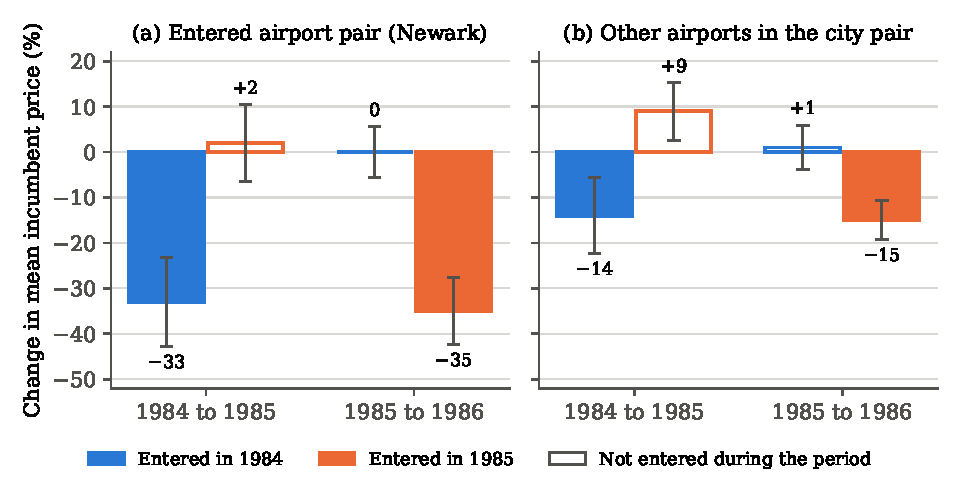
\includegraphics[width=\linewidth]{figures/ch09/wc_did.pdf}
\caption{Percentage change in the mean incumbent price by entry cohort and period. Filled bars are the
cohort entered during the period, and open bars the cohort not entered during it. Whiskers show plus
or minus one standard error of the cohort mean, computed as the reported cross-market standard
deviation divided by $\sqrt{n}$ ($n=7$ and $8$). Redrawn from \citet{WhinstonCollins1992}, Tables~3
and~4.}
\label{fig:09-wc-did}
\end{figure}

\casehead{Prices}
The pattern is similar in the two periods (p.~459). In markets entered during a
year, the mean incumbent price fell by about 35 percent. In markets not entered that year it barely
moved. The two contrasts are $-35$ points each, with $t$ statistics of 2.5 and 3.5. Their equality is
consistent with the three assumptions. So are the 2 percent rise in the 1985 cohort's prices before
its entry and the flat prices of the 1984 cohort in the year after its entry. None of these patterns
confirms the assumptions, because offsetting departures from them reproduce all four changes. Suppose the true
effect is $-25$ points and fades by 10 points in its second year. Suppose also that, without entry,
prices in the 1984 cohort would have fallen 10 points more than in the 1985 cohort in 1984--1985. Let
prices in the 1985 cohort rise 2 points in 1984--1985, as observed. Let all prices fall 10 points in 1985--1986 for reasons unrelated to entry. These values give exactly the
changes $-33$, $+2$, $0$ and $-35$ of Panel~A. Even after the cuts, People Express's average fare in the first
quarter after entry was 19 percent below the incumbents' mean fare.

Price dispersion fell, or rose less, in entered markets. The contrast is larger in 1984--1985 ($-55$
points, $t=2.6$) than in 1985--1986 ($-20$ points, $t=1.0$). The authors speculate that airlines grew
more skilled at \emph{yield management}, the dynamic allocation of seats across fare classes, over the
period. By 1985--1986 an incumbent could target its price
cuts where they mattered most, without lowering all fares.

\casehead{Quantities and revenue}
Incumbents sold more tickets after entry, if anything. The contrasts are $+72$ and $+74$ points, but
the variation across markets is large and neither is significant. Revenue fell much less than the price
cuts alone would imply (n.~34). In 1984--1985, revenue in entered markets rose 21 percent (s.d.\
22) against 33 percent (s.d.\ 28) in markets not entered. In 1985--1986 the figures are 3 percent
(s.d.\ 29) and 10 percent (s.d.\ 16). Revenue understates the incumbents' loss, because carrying more
passengers raises costs and, as we see next, incumbents also added capacity.

\casehead{Capacity}
The authors compared incumbents' nonstop seats on the entered route one year after the announcement
with seats at the announcement, using the \emph{Official Airline Guide}. Seats rose 25 percent on
average (s.d.\ 42). Domestic seats at Newark offered by carriers other than People Express rose 11
percent a year over 1984--1986. That benchmark includes the entered markets, so the comparison
understates the gap (n.~35). Nearly all of the increase came from flight frequency. Seats per
flight rose only 6 percent (s.d.\ 20), against 3 percent at Newark. The capacity increases were larger
for the 1984 cohort, 48 percent (s.d.\ 52), than for the 1985 cohort, 5 percent (s.d.\ 14)
(n.~36).

\casehead{Other airports in the city pair}
Panel~B shows the same pattern on a smaller scale (pp.~460--461). Prices fell 14 and 15 percent
in the treated cohorts, the ``15\%'' the paper quotes, while the control cohorts' prices rose 9 and 1
percent. The contrasts are $-23$ points ($t=2.1$) and $-16$ points ($t=2.3$). Quantity changes are
small and insignificant. Incumbent capacity on these routes rose 1 percent (s.d.\ 30) in the year
after entry, against a 1 percent decline at Kennedy and La Guardia. Seats per flight fell 4 percent
(s.d.\ 9), against a 2 percent decline at those airports, so frequency again rose. Price dispersion
again fell relative to controls, more in 1984 than in 1985. The smaller price response matches the
small $\mathit{OSM}$ value effect. Airports in a city are substitutes, but imperfect ones.

\casehead{Interpretation}
The quantity and capacity responses discriminate among models of competition (p.~460). Under
price taking, each incumbent sells where price equals its marginal cost. Entry lowers the market price
and moves each incumbent down its supply curve, so its output falls. Price cuts together with rising
sales and capacity are hard to square with any simple price-taking model. The rents revealed by the
value losses are therefore not the efficiency rents of a competitive market.

Static oligopoly models predict the same direction as price taking. In symmetric Cournot competition
each firm's output falls when the number of firms rises \eqref{eq:09-cournot-entry}, and by
\cref{rem:09-ks} the same holds for capacities. By \eqref{eq:09-br-slope}, the observed responses fit
static models only if quantities are strategic complements, which requires unusually convex demand.
They are consistent with a dynamic strategy. Industry observers
claimed that incumbents responded aggressively to induce exit, or at least to discourage further
expansion. The larger capacity increases in 1984 fit this interpretation. The responses also show that
the value losses did not reflect a temporary adjustment toward a smaller scale of operations.

The authors add a caution (pp.~458--459). Demand or cost conditions may have changed in the
entered markets, and such changes might even have caused entry. The size of the effects and the view
that the events reflected People Express's own strategy make it plausible that most of the change is
a response to entry.

\subsection{Conclusions, limitations, and contribution}\label{sec:09-wc-concl}

\casehead{What the paper concludes, and where}
\Cref{tab:09-wc-claims} lists each conclusion of the paper with the evidence and the test behind it.
The value results come from the $\mathit{SM}$ rows of \cref{tab:09-wc-t1,tab:09-wc-t2}. The contrast
between airports comes from the $\mathit{OSM}$ rows and the test of equal effects. The general effects
come from the fixed-effect sums. The incumbent responses come from \cref{tab:09-wc-t34} and the
schedule comparisons.

\begin{table}[htbp]
\centering
\caption{Conclusions of Whinston and Collins (1992) and the supporting evidence}
\label{tab:09-wc-claims}
\footnotesize
\begin{tabularx}{\linewidth}{@{}>{\raggedright\arraybackslash}p{0.27\linewidth}
  >{\raggedright\arraybackslash}X >{\raggedright\arraybackslash}p{0.25\linewidth}@{}}
\toprule
Conclusion & Evidence & Test\\
\midrule
Route-specific profits or sunk costs exist, so airline routes are not contestable &
$\lambda_{SM}<0$ in all windows (Table 1) and all specifications (Table 2, SM row). Loss of \$3.7 to
\$6.5 million per incumbent & $t$ tests of $\lambda_{SM}=0$: $-2.98$ to $-3.15$ (Table 1), $-2.18$
(Table 2, column 5)\\
\addlinespace
Local market structure matters, and profits are not equalized across routes &
Incumbency loss survives firm fixed effects. An incumbent loses \$6.2 million versus \$1.9 million
for a non-incumbent (Table 2, column 5) & $t$ test of $\lambda_{SM}$ with fixed effects, fixed-effect
sum\\
\addlinespace
Airports in the same city are differentiated &
$\lambda_{OSM}$ small, positive, insignificant (Table 2, columns 3 to 5) & Test of
$\lambda_{SM}=\lambda_{OSM}$, rejected at 2.5 percent\\
\addlinespace
Large industry-wide effects of unclear origin & Sum of fixed effects $-\$36.2$ million, over 80
percent of industry loss (Table 2, column 5) & Standard error of the sum, quasi-likelihood ratio test
of New York versus other fixed effects\\
\addlinespace
Incumbents cut prices sharply but raised capacity and sales &
Price contrasts of $-35$ points on the entered pair and $-23$ and $-16$ at other airports. Seats $+25$
percent (Tables 3 and 4, schedule data) & Two-sample $t$ tests with 13 degrees of freedom\\
\bottomrule
\end{tabularx}

\smallskip
\parbox{0.97\linewidth}{\footnotesize Notes: Table numbers refer to \citet{WhinstonCollins1992}, reproduced
here as \cref{tab:09-wc-t1,tab:09-wc-t2,tab:09-wc-t34}.}
\end{table}

\casehead{From descriptive results to economic inferences}
The chain of reasoning has three links. The first is statistical. Incumbents' abnormal dollar
changes on announcement days are negative and proportional to their seat-miles on the entered route.
The second is the efficient-markets link. Under (E1) to (E5) the abnormal change equals the change in
expected discounted profits caused by the news. The third is theoretical. By \cref{prop:09-valueloss},
a loss of expected profits from entry implies pre-entry rents or sunk costs, which contestability
excludes. Each richer specification in \cref{tab:09-wc-t2} rules out an alternative reading of the
first link. Slot rents at nearby airports, general industry effects and connecting markets cannot
account for the incumbency loss.

\casehead{Advantages over pricing regressions}
The event study needs no model of the network, and no controls for each route's demand and cost.
The variation comes from the timing of announcements and from incumbents' exposure, which People
Express's strategy determined. The method also measures the level of rents in dollars, as a lower
bound, where a pricing regression delivers a correlation between fares and structure.

\casehead{Limitations}
The design has several limitations, some noted by the authors and some raised by the logic of the
method.
\begin{itemize}
\item The sample is small. There are 24 events on 17 dates, and 22 involve Newark. The general effects
use 19 parameters, and the non-New York effects rest on two events.
\item Dating and anticipation bias the estimates toward zero. People Express's expansion was public
and ongoing, so markets probably expected some entry. Later work on Southwest finds that incumbents cut
fares once entry becomes likely, before the entrant starts flying \citep{GoolsbeeSyverson2008}. News
about entry can therefore arrive well before any announcement.
\item The general effects remain unexplained. Information about People Express's future scale,
competitive spillovers and aircraft values cannot be separated. If informational effects are
correlated with incumbency, part of the $\mathit{SM}$ effect could be informational. The separate New
York effects address this only partly.
\item Entry into a carrier's markets might signal that People Express intended to ``go after'' that
carrier. This informational effect would also load on incumbency. The authors see no way to control for
it without strong assumptions about its form, and they find little evidence of such a pattern (n.~25).
\item Seat-miles measure capacity. They do not count passengers. Connecting traffic is not controlled for, and the
loss per seat is assumed common across routes up to the robustness checks of footnote~32.
\item The bound $L\le V^0+K$ cannot separate pre-entry profits from sunk costs. The value change also
embeds the expected post-entry game, including the incumbents' own aggressive responses.
\item External validity is limited. People Express was a special entrant, with a new low-frill product
and low labor costs, in a transitional period after deregulation.
\item The price and capacity evidence uses 7 and 8 markets, with no formal control for changes in
demand. Only one year precedes the entry of both cohorts. The design therefore cannot separate
differential trends from effects that change after entry, and offsetting departures pass its one
testable restriction. If incumbents moved aircraft from control markets into entered markets, the control group is
affected by entry and the quantity contrasts are overstated.
\end{itemize}

\casehead{Contribution}
\citet{WhinstonCollins1992} gave a market-based test of contestability that does not depend on
controls for route demand and cost. Their incumbency loss confirms the conclusion of the pricing
studies that local structure matters, and it adds a dollar measure of rents. They gave market-based
evidence that airports serving the same city are differentiated, and they documented large
industry-wide effects of entry announcements. Their price and capacity evidence showed incumbents
responding to a low-fare entrant with deep price cuts and more capacity. The abnormal-dollar
formulation, with exposure measures that vary across firms, carries over to event studies of mergers
(\cref{ch:mergers}). \Cref{sec:09-synthesis} compares what this design identifies with the pricing
regressions of \cref{sec:09-borenstein} and the structural model of \cref{sec:09-bcs}.
